\documentclass{article}
\usepackage{preambule}

\begin{document}

\newcommand{\spp}{superpixel}

\begin{center}
    \begin{Large}\textbf{IMAGE SEGMENTATION BY SUPERPIXELS}\end{Large}

    \vspace{1cm}
    \begin{large}\textbf{\underline{T.Dumont$^a$}, B.Figliuzzi$^b$}\end{large}

    \vspace{0.5cm}
    a. MINES ParisTech, theo.dumont@mines-paristech.fr\\
    b. MINES ParisTech CMM, bruno.figliuzzi@mines-paristech.fr
    \vspace{1cm}
\end{center}

\begin{center}
\noindent\textbf{Key-words: }\\
deep learning; convolutional neural networks; image segmentation\\
\ \\
\textbf{Abstract: }\\
In this paper, we study different options to improve the performance of a deep learning convolutional neural network
\end{center}

\tableofcontents

\section*{Todo}
\begin{itemize}
    \item
\end{itemize}

\newpage
\section{Introduction}

    \subsection{Segmentation}
            \paragraph{What it is}piche

            \begin{figure}[!htb]
                \centering
                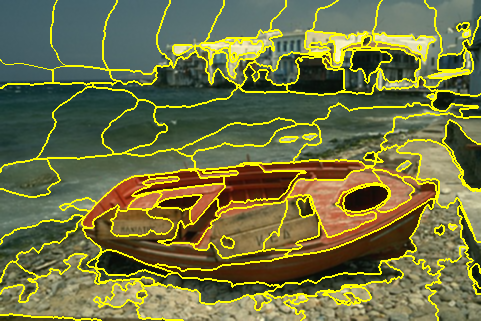
\includegraphics[scale=0.5]{pics/img.png}
                \caption{\textit{An image and its segmented image}}
                \label{fig:segm}
            \end{figure}
            \paragraph{Motivation}

    \subsection{Superpixels}
            \paragraph{What it is}piche

            \begin{figure}[!htb]
                \centering
                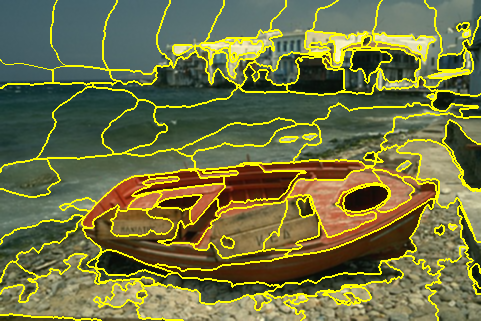
\includegraphics[scale=0.5]{pics/img.png}
                \caption{\textit{Partition d'une image en superpixels}}
                \label{fig:spp}
            \end{figure}

            \paragraph{Applications \& Motivation}
            démarrer une segmentation\\
            fournir un support sur lequel faire de la classification (couleur/texture moyenne, etc)


    \subsection{Ce qu'est une bonne \spp segmentation}
        \subsubsection{Metrics}
            \paragraph{metric1}
            \paragraph{metric1}
            \paragraph{metric1}
            \paragraph{metric1}

        \subsubsection{SLIC}
        \subsubsection{Autres algorithmes}

    \subsection{Motivations/ambitions}
            \paragraph{Difficultés que l'on cherche à résoudre}
            \paragraph{Pas de vraie approche DL pour segmentation avec \spp s}
            \paragraph{Ambitions}
            améliorer les métriques









\section{Dataset generation}
    \subsection{COCO dataset}
        \subsubsection{The COCO dataset}
        COCO dataset
        \subsubsection{Characteristics}
        \label{par:charac}

        max, min pixels, etc
        graphes pour décrire les données
    \subsection{Eikonal}
    \subsection{Notre utilisation de eikonal}
    en plus réutilisé derrière sur image qui sort du réseau\\
    faire un petit résumé









\section{The model}
    \subsection{Approach}
    description générale de l'approche (NN puis eikonal)
    \subsection{Network architecture}
        \subsubsection{Layers definitions}

            \paragraph{Dilated convolution}\label{par:dilated} We consider a layer $L=(L_j)_{j\in [\![1,w]\!]}$, $w$ being the number of feature maps $L_j$ of $L$. We also consider $K=(K_{i,j})_{i,j}$, each $K_{i,j}$ being a $3\times 3$ convolutional kernel. The dilated convolution operation of $K_{i,j}$ on $L_j$ is denoted by $L_j*_r K_{i,j}$, $r$ being the dilation parameter.
            \begin{figure}
                \begin{subfigure}{.49\linewidth}
                    \centering
                    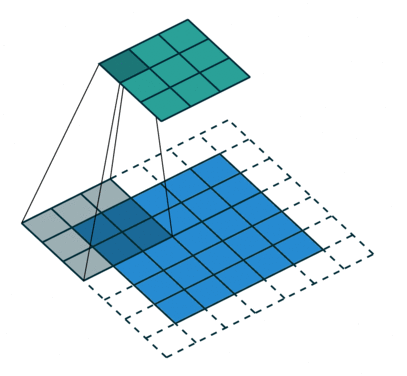
\includegraphics[width=.8\linewidth]{pics/conv-simple.png}
                    \caption{\textit{A simple convolution ($r=1$)}}
                    \label{fig:conv-simple}
                \end{subfigure}
                \begin{subfigure}{.49\linewidth}
                    \centering
                    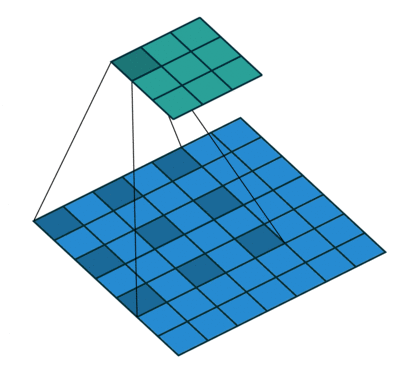
\includegraphics[width=.8\linewidth]{pics/conv-dilated.png}
                    \caption{\textit{A dilated convolution ($r=2$)}}
                    \label{fig:conv-dilated}
                \end{subfigure}
                \caption{\textit{Illustration of two types of convolutions}}
            \end{figure}
            The output $C(x)$ of a pixel $x$ is:
            \begin{flalign*}
            C(x):& = (L_j*_r K_{i,j})(x) &\\
                 & = \sum_{a+rb=x}L_j(a)K_{i,j}(b) &\\
                 & = \sum_b L_j(x-rb)K_{i,j}(b) &
            \end{flalign*}
            and we recognize the simple convolution when $r=1$.\\
            A dilated convolution enables the network getting larger receptive fields while preserving the input resolution\footnote{ref ?}


            \paragraph{Adaptative Batch Normalization (ABN)} As we have seen in (\ref{par:charac}), page \pageref{par:charac}, we need to normalize the data. We define the \textit{adaptative normalization function} $\Psi$ as:
            $$\Psi(x)=a\ x+b\ BN(x),$$
            where $BN$ is the classic batch normalization\footnote{reference ?}, defined as:
            $$BN(x) = \frac{x-\mathrm{E}[x]}{\sqrt{\mathrm{Var}[x]+\epsilon}}*\gamma+\beta.$$
            As such, $\Psi$ combines identity mapping and batch normalization. $a$, $b$, $\gamma$ and $\beta$ are learned parameters\footnote{ref : \url{https://pytorch.org/docs/stable/_modules/torch/nn/modules/batchnorm.html}} by backpropagation. It allows the model to adapt to each dataset, choosing whether or not giving a big importance to the identity term and the normalization term.

            \paragraph{Leaky rectifier (LReLU)} In order to let our neural network model complex patterns in the data, we have to add a non-linear property to the model. It often is an activation function, such as a sigmoid or a tanh (Figure \ref{fig:act-sigmoids}).

            \begin{figure}
                \begin{subfigure}{.49\linewidth}
                    \centering
                    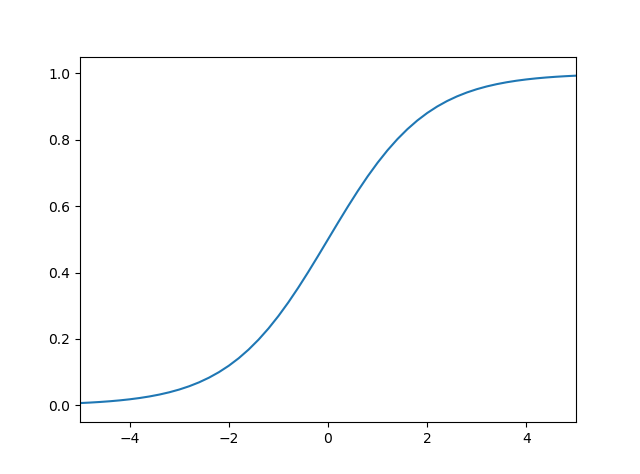
\includegraphics[width=\linewidth]{pics/act-sigmoid.png}
                    \caption{\textit{Sigmoid}}
                \end{subfigure}
                \begin{subfigure}{.49\linewidth}
                    \centering
                    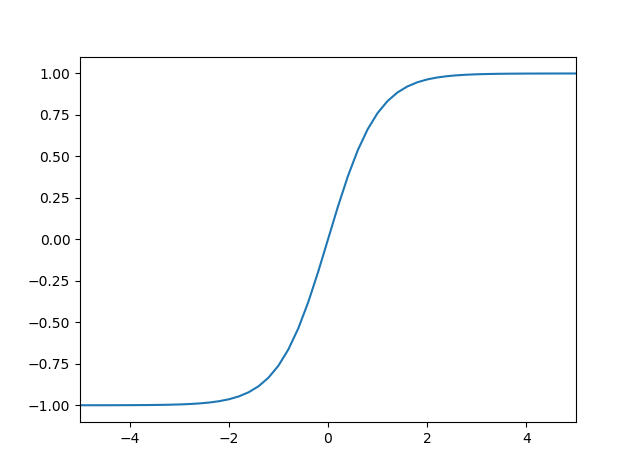
\includegraphics[width=\linewidth]{pics/act-tanh.png}
                    \caption{\textit{tanh}}
                \end{subfigure}
                \caption{\textit{Illustration of two bounded rectifiers}}
                \label{fig:act-sigmoids}
            \end{figure}

            The problem with these activation functions is that they are bounded and their gradient is very low on the edges. Because we want are going to manipulate high scalar values, we have to use an unbounded activation function, such as ReLU, $\Phi(x)=\max(0,x)$ (Figure \ref{fig:relu}). But the issue with ReLU is that all the negative values become zero immediately, which decreases the ability of our model to train from the data. Hence the implementation of a \textit{leaky rectifier}, LReLU:
            $$\Phi(x)=\max(\alpha x,x)\mbox{, with } 0<\alpha<1.$$

            \begin{figure}
                \begin{subfigure}{.49\linewidth}
                    \centering
                    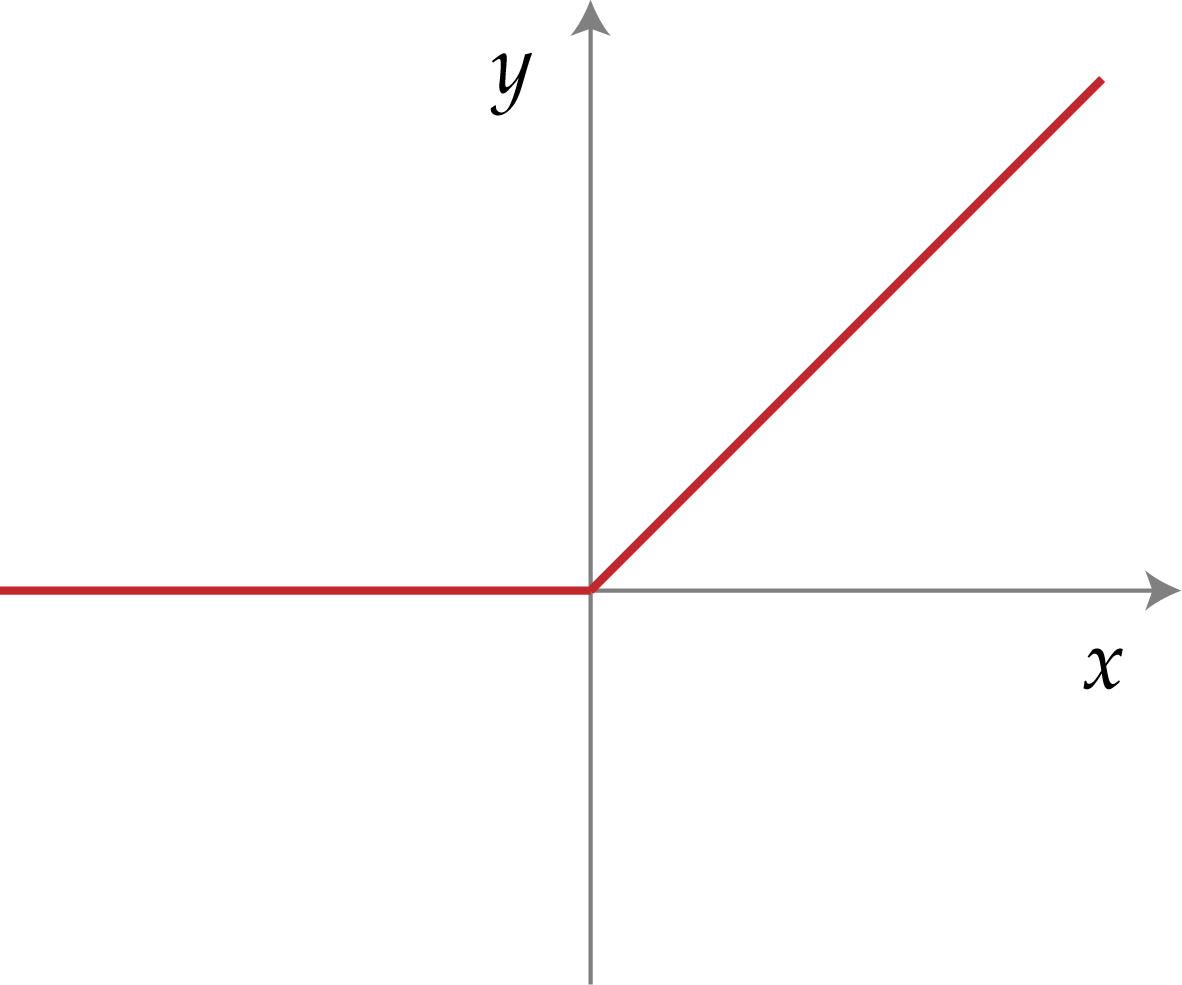
\includegraphics[width=.8\linewidth]{pics/act-relu.png}
                    \caption{\textit{ReLU}}
                    \label{fig:relu}
                \end{subfigure}
                \begin{subfigure}{.49\linewidth}
                    \centering
                    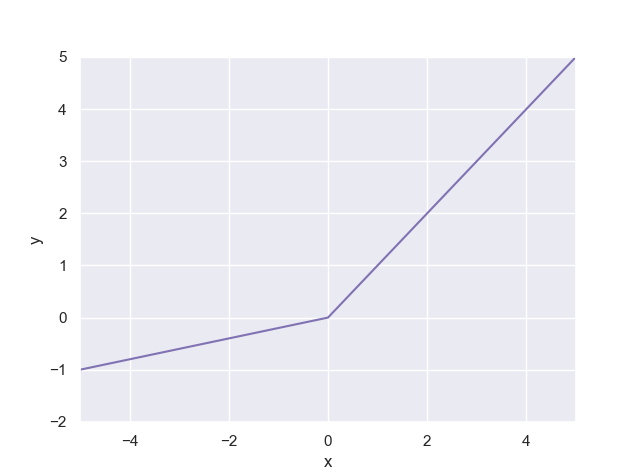
\includegraphics[width=.8\linewidth]{pics/act-lrelu.png}
                    \caption{\textit{LReLU ($\alpha=0.2$)}}
                    \label{fig:lrelu}
                \end{subfigure}
                \caption{\textit{Illustration of two unbounded rectifiers}}
            \end{figure}

            By implementing a Leaky Rectifier, we are able to take into account the negative valued pixels.



        \subsubsection{Chen}
            \paragraph{Context Aggregation Network (CAN)}\footnote{reference}
            \begin{table}[!ht]
                \center
                \begin{tabular}{ccccccccccc}
                    \hline
                    input $I$ & $\longrightarrow$ & $L^1$ & $\longrightarrow$ & $\cdots$ & $\longrightarrow$ & $L^s$ & $\longrightarrow$ & $\cdots$ & $\longrightarrow$ & output ($L^d$)\\
                    $m\times n\times 3$ & & $m\times n\times w_1$ & & & & $m\times n\times w_s$ & & & & $m\times n\times 3$\\
                    \hline
                \end{tabular}
                \caption{\textit{Layers}}
            \end{table}
            blabla sur le RGB en entrée, RGB en sortie I -> f(I)
            \paragraph{Architecture of a block}
            Each block $L_s$ is made of 3 layers:
            \begin{enumerate}
                \item \textit{A dilated convolution}, $r_s=2^s$
                \item \textit{An adaptative batch normalization}
                \item \textit{A leaky rectifier (ReLU)}
            \end{enumerate}
            so that the content of an intermediate layer $L^s$ can be computed from the content of the previous layer $L^{s-1}$:
            \begin{equation}
                L_i^s=\Phi\left(\Psi^s\left(b_i^s+\sum_jL_j^{s-1}*_{r_s}K^s_{i,j}\right)\right).
            \end{equation}
            where ... is ...

            and
            \begin{equation}
                L_j^{s-1}*_{r_s}K^s_{i,j}=\sum_{a+r_sb=x}L_j^{s-1}(a)K_{i,j}^s(b)
            \end{equation}
            because of \ref{par:dilated}, page \pageref{par:dilated}.

            \begin{table}[!ht]
                \center
                \begin{tabular}{|c|c|c|c|c|c|c|c|}
                    \hline
                    Layer & 1 & 2 & 3 & 4 & 5 & 6 & 7\\
                    \hline \hline
                    Convolution & $3\times3$ & & & & & & \\
                    \hline
                    Dilation & 1 & & & & & & \\
                    \hline
                    Batch Normalization & Yes & & & & & & \\
                    \hline
                    LReLU & Yes & & & & & & \\
                    \hline
                \end{tabular}
                \caption{\textit{Chen}}
            \end{table}

        \subsubsection{UNet}
        \subsubsection{Chen + UNet}

    \subsection{Total Variation (TV) Loss}
        \subsubsection{MSE}
        \subsubsection{TV}
            \paragraph{Formula}
            \paragraph{Why}

est-ce que l'on parle de la façon dont on compute le gradient et des différentes méthodes que l'on a essayées

    \subsection{Implementation}
    The network was implemented with PyTorch\footnote{Repository can be found at \url{https://github.com/theodumont/superpixels-segmentation}.} and we used GPU acceleration [...]
    (pytorch), se renseigner (section assez courante)
    GPU acceleraation
    code sur github









\section{Expérience et résultats}
    \subsection{Hyperparameters}
    évolution des paramètres a et b ?\\
    entrainement (lr, alpha) -> courbes de loss, et loss qui sature (cluster) d'où changement de lr au cours des epochs
    nb epochs: on le sélectionne en prenant le minimum de la validation loss
        \subsubsection{Runs}
        tableaux et graphes
    \subsection{Results on dataset}
    image originale -> CNN -> résultat du filtre dans eikonal -> superpixels sans couleurs + couleur moyenne pour chaque spp de l'image originale
    cf results/images











\section{Conclusion/Discussion}
On a présenté un nouveau...\\
On a prouvé...\\
Il reste à faire...

relire tous les mails pour avoir toutes les infos sur performances etc

\section*{Special thanks}

\section*{Sources}

\noindent
{[}1]
{[}1] C. Smith, J.C. Green, Titre de l’article, Titre du journal, 10 (2009) 55-72\\
{[}2] M. Truk, C. Bidul. Titre du bouquin, John Wiley and Sons, New York, 1973\\
{[}3] P. Machin, Titre de la thèse, Thèse, Université Poitiers, 1992\\
{[}4] D. Pierre, J.-P. Paul, B. Jacques, Titre communication, in: D. Editor, G. Editeur, ( éd.), Proceedings of Conference XXX , Publisher, Paris, France, 1995, pp. 3–6

\newpage


\end{document}
